% ch1-hermite.tex
\documentclass[../main/main]{subfiles}

\begin{document}

\chapter{Hermite多項式}
\footnotesize
Hermite多項式は量子力学で調和振動子の問題を扱う際に解として現れる関数である( 問題[1-1] )。
本稿で扱う特殊関数のうち最もなじみやすい関数でもあり、
その公式の導出手順は他の特殊関数に適用することが可能である。
そこでまず本章のHermite多項式を題材に特殊関数の取り扱い方に慣れていきたい。
ここで技術を身につけておくと他の特殊関数も自然と理解しやすくなる。

\small
\section{Hermite多項式}

\subsection*{公式集}

\small
\paragraph{母関数}
\begin{equation}\label{eq:Hn-gene}
  g(t, x) = e^{-t^2+2xt} = \sum_{n=0}^\infty \frac{t^n}{n!} H_n(x)
\end{equation}

\paragraph{偶奇性}
\begin{equation}
  H_n(-x) = (-1)^n H_n(x)
\end{equation}

\paragraph{$x=0$での特殊値}
\begin{subnumcases}{}
  H_{2n} (0) = (-1)^n \frac{(2n)!}{n!} & \\
  H_{2n+1} (0) = 0 
\end{subnumcases}

\paragraph{一般項}
\begin{equation}
  H_n(x) = \sum_{i=0}^{\lfloor \frac{n}{2} \rfloor} (-1)^i \frac{n!}{i! (n-2i)!} (2x)^{n-2i}
\end{equation}

\paragraph{Rodriguesの公式}
\begin{equation}\label{Hn-Rod}
  H_n(x) = (-1)^n e^{x^2} \dx{n} e^{-x^2}
\end{equation}

\paragraph{漸化式}
\begin{equation}\label{eq:Hn-req}
  H_{n+1}(x) = 2x H_n(x) - 2n H_{n-1} (x)
\end{equation}

\paragraph{昇降演算子}
\begin{alignat}{2}
  &\textbf{下降演算子} &\qquad	& \dx{} H_n (x) = 2n H_{n-1} (x) \label{eq:Hn-kako} \\
  &\textbf{上昇演算子} &		& \( \dx{} -2x \) H_n(x) = - H_{n+1}(x) \label{eq:Hn-josho}
\end{alignat}


\paragraph{微分方程式}
\begin{equation}
  \frac{d^2 H_n (x)}{dx^2} - 2x \frac{d H_n(x)}{dx} + 2n H_n(x) = 0
\end{equation}

\paragraph{自己随伴形}
\begin{equation}
  \dx{} \( e^{-x^2} \dx{}H_n(x) \) + 2n  e^{-x^2} H_n(x) = 0
\end{equation}

\paragraph{直交性}
\begin{equation}
  \int_{-\infty}^\infty e^{-x^2} H_m(x) H_n(x) \, dx = 2^n n! \sqrt{\pi} \, \delta_{mn}
\end{equation}


\vspace{-12pt}
\begin{figure}[tb]
\begin{tabular}{cc}
 \begin{minipage}{0.45\hsize}\small
    \begin{table}[H]
      \centering
      \small
      \caption{Hermite多項式$H_n(x)$}
      \begin{tabular}{ccl}\Hline
        $H_0(x)$ & $=$ & $1$ \\
        $H_1(x)$ & $=$ & $2x$ \\
        $H_2(x)$ & $=$ & $4x^2-2$ \\
        $H_3(x)$ & $=$ & $8x^3-12x$ \\
        $H_4(x)$ & $=$ & $16x^4 - 48x^2 + 12$ \\
        $H_5(x)$ & $=$ & $32x^5 - 160x^3 + 120x$ \\
        $H_6(x)$ & $=$ & $64x^6 - 480x^4 + 720x^2 - 120$ \\\hline
      \end{tabular}
    \end{table}
 \end{minipage}

 \begin{minipage}{0.55\hsize}
      \centering
      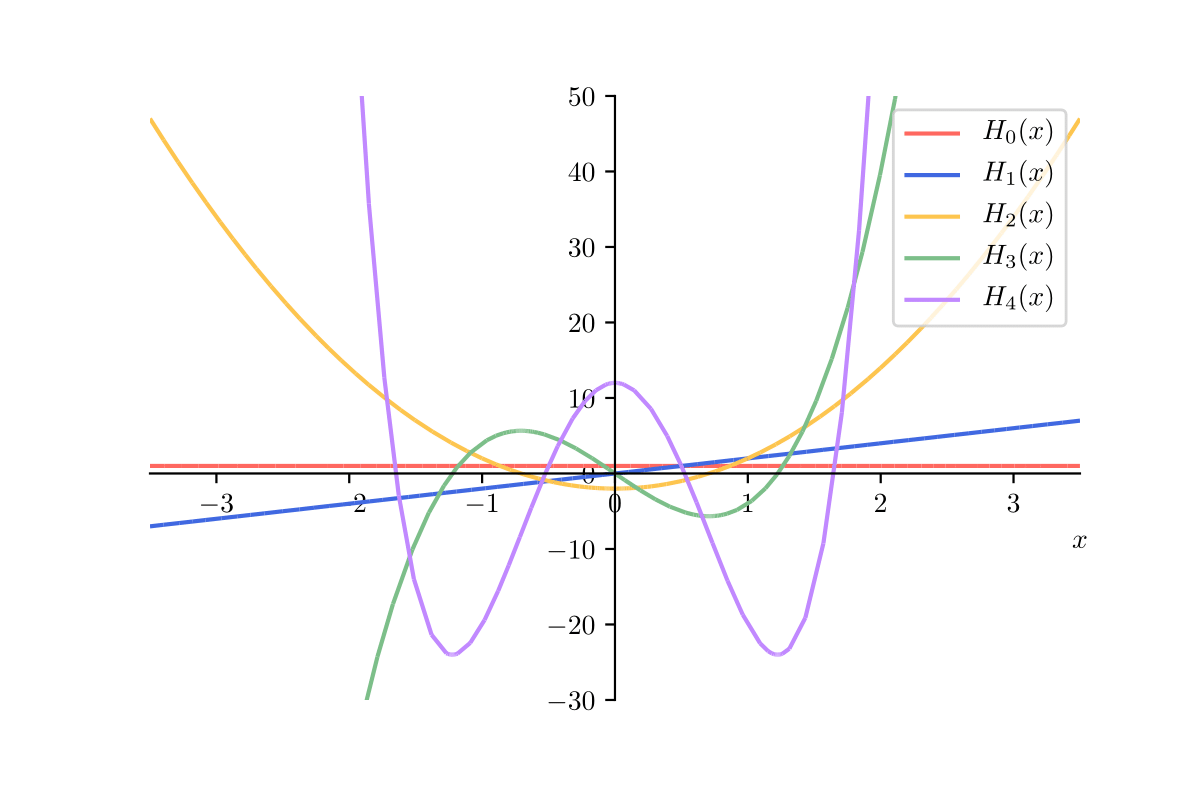
\includegraphics[width=90mm]{../fig/hermite/hermite.png}\vspace{-24pt}
      \caption{Hermite多項式$H_n(x)$}
  \end{minipage}
\end{tabular}
\end{figure}

\subsection*{証明}
\paragraph{母関数 $\Longrightarrow$ 偶奇性}
母関数\eqref{eq:Hn-gene}の中辺から$g(-t, -x) =g(t, x)$が成立することが分かるので、
\eqref{eq:Hn-gene}の右辺から
\begin{equation*}
  \sum_{n=0}^\infty \frac{(-t)^n}{n!} H_n(-x) = \sum_{n=0}^\infty \frac{t^n}{n!} H_n(x)
\end{equation*}
$t^n \ (n\geq 0)$の係数を比較して、
\begin{equation*}
  H_n(-x) = (-1)^n H_n(x)
\end{equation*}\qed

\paragraph{母関数 $\Longrightarrow$ $x=0$での特殊値}
母関数\eqref{eq:Hn-gene}に$x=0$を代入すると、
\begin{equation}\label{eq:Hn-gen->x=0-En}
  g(t, 0) = e^{-t^2} = \sum_{n=0}^\infty \frac{t^n}{n!} H_n(0)
\end{equation}
ここで、\eqref{eq:Hn-gen->x=0-En}の中辺をTaylor展開すると、
\begin{equation}\label{eq:Hn-gen->x=0-En-1}
  e^{-t^2} = \sum_{n=0}^\infty \frac{(-t^2)^n}{n!}
	= \sum_{n=0}^\infty (-1)^n \frac{t^{2n}}{n!}
\end{equation}
一方\eqref{eq:Hn-gen->x=0-En}の右辺は
\begin{equation}\label{eq:Hn-gen->x=0-En-2}
  \sum_{n=0}^\infty \frac{t^n}{n!} H_n(0)
	= \sum_{n=0}^\infty \frac{t^{2n}}{(2n)!} H_{2n}(0)
		+ \sum_{n=0}^\infty \frac{t^{2n+1}}{(2n+1)!} H_{2n+1}(0)
\end{equation}
と分解できる。
\eqref{eq:Hn-gen->x=0-En-1}と\eqref{eq:Hn-gen->x=0-En-2}より
$t^n \ (n\geq 0)$の係数を比較して、次が得られる。
\begin{subnumcases}{}
  H_{2n} (0) = (-1)^n \frac{(2n)!}{n!} & \notag\\
  H_{2n+1} (0) = 0 \notag
\end{subnumcases}\qed

\paragraph{母関数 $\Longrightarrow$ Rodriguesの公式}
母関数\eqref{eq:Hn-gene}の中辺を、$x$を固定して$t=0$の周りでTaylor展開すると、
\begin{equation}
  g(t, x) = e^{x^2} e^{-(t-x)^2} 
	= e^{x^2} \sum_{n=0}^\infty \frac{t^n}{n!} \[ \dt{n} e^{-(t-x)^2} \]_{t=0} \notag
\end{equation}
  {ここで$t-x = u$とおくと、$dt = du$であることから}
\begin{align}
  g(t,x) &= e^{x^2} \sum_{n=0}^\infty \frac{t^n}{n!} \[ \frac{d^n}{du^n} e^{-u^2} \]_{u=-x} \notag\\
	&= e^{x^2} \sum_{n=0}^\infty \frac{t^n}{n!} \frac{d^n}{d(-x)^n} e^{-(-x)^2} \notag\\
	&=  \sum_{n=0}^\infty \frac{t^n}{n!} (-1)^n e^{x^2} \frac{d^n}{dx^n} e^{-x^2} \notag
\end{align}
となる
\footnote{ここで用いたテクニックはやや技巧的だが大幅に計算量を減らすことができている。
覚えておくことを推奨する。}。
これと\eqref{eq:Hn-gene}の右辺を比較することで次を得る。
\begin{equation*}
  H_n(x) = (-1)^n e^{x^2} \dx{n} e^{-x^2}
\end{equation*}\qed

\paragraph{Rodrigues公式 $\Longrightarrow$ 母関数}

Cauchyの積分公式
\footnote{
\textbf{Cauchyの積分公式}: 正の向きを持つ区分的に滑らかなJordan曲線$C$上の点と内部で
正則な関数$f(z)$について、点$x$が$C$の内部にあるとき
\begin{equation}\label{eq:cauchy}
  f(x) = \frac{1}{2\pi i} \int_C \frac{f(\xi )}{\xi - x} d\xi  
\end{equation}
と書けるという定理である。本文中ではこの両辺を$x$について$n$回微分した、
以下の$n$階導関数を積分で表す公式を用いている。
\begin{equation}\label{eq:cauchy-diff}
  f^{(n)} (x) = \frac{n!}{2\pi i} \int_C \frac{f(\xi )}{(\xi -x)^{n+1}} d \xi 
\end{equation}
}
を用いてRodriguesの公式\eqref{Hn-Rod}を積分形式に書き換えると、
\begin{equation*}
  H_n(x) = (-1)^n e^{x^2} \cdot \frac{n!}{2\pi i} \int_C \frac{e^{-\xi^2}}{(\xi - x)^{n+1}} d\xi
\end{equation*}
ここで積分経路$C$は$\xi=x$の周りを正の方向に回るようにとる。
よって、
\begin{align}
  \sum_{n=0}^\infty \frac{t^n}{n!} H_n(x)
	&= \sum_{n=0}^\infty \frac{t^n}{n!} \cdot
		(-1)^n e^{x^2} \cdot \frac{n!}{2\pi i} \int_C \frac{e^{-\xi^2}}{(\xi - x)^{n+1}} d\xi \notag\\
	&= e^{x^2}  \frac{1}{2\pi i} 
		\int_C \frac{e^{-\xi^2}}{\xi-x} \sum_{n=0}^\infty \( \frac{-t}{\xi-x} \)^n d\xi \notag
\end{align}
級数が収束するために$|t|$が十分小さいものとすると、等比級数の和の公式から
\begin{align}
  \sum_{n=0}^\infty \frac{t^n}{n!} H_n(x)
	&= e^{x^2} \frac{1}{2\pi i} 
		\int_C \frac{e^{-\xi^2}}{\xi-x} \cdot \frac{1}{1 + \frac{t}{\xi-x} } d\xi \notag\\
	&= e^{x^2} \frac{1}{2\pi i} \int_C
		\frac{e^{-\xi^2}}{\xi - (x-t)} d\xi \notag
\end{align}
被積分関数の極$\xi=x-t$が、$t$が十分小さく、$C$の内部にあるとすると、留数定理より
\begin{equation*}
  \sum_{n=0}^\infty \frac{t^n}{n!} H_n(x) 
	= e^{x^2} \frac{1}{2\pi i} \cdot 2\pi i \[ e^{-\xi^2} \]_{\xi = x-t}
	= e^{-t^2+ 2xt}
\end{equation*}\qed



\paragraph{母関数 $\Longrightarrow$ 一般項}
母関数\eqref{eq:Hn-gene}の中辺を$e^x = \sum_{i=0}^\infty \frac{1}{i!} x^i$を用いて展開すると、
\begin{align}
  g(t, x) &= e^{-t^2+2xt} 
	= \sum_{m=0}^\infty \frac{1}{m!} (-t^2+2xt)^m \notag\\
	&= \sum_{m=0}^\infty \frac{1}{m!} \sum_{i=0}^m \binom{m}{i} (-t^2)^i (2xt)^{m-i}
		\qquad (\since 二項定理)\notag\\
	&=\sum_{m=0}^\infty \sum_{i=0}^m  t^{m+i} \, (-1)^i \frac{1}{i! (m-i)!} (2x)^{m-i}
		\label{eq:Hn-gene->ippan}
\end{align}


\vspace{-12pt}
\begin{figure}[H]
  \begin{tabular}{c}
 \begin{minipage}{0.54\hsize}\small
ここで$m+i$を新たに$n$と置き換えて$m, i$についての二重和を$n, i$についての二重和に取りかえる。
$m$について$0$から$\infty$まで、$i$について$0$から$m$まで加えていくとき、
二重和は図\ref{fig:hermite}の黒丸で表した格子点すべてについて実行される。
$n=m+i$であるとき、$n=0, 1, 2, \dots$に対応する全格子点は
図\ref{fig:hermite}で示した各矢印上の点として捉えることができる。
したがって図\ref{fig:hermite}より、\eqref{eq:Hn-gene->ippan}における二重和は、
$n$について$0$から$\infty$まで、$i$について$0$から$\lfloor \frac{n}{2} \rfloor$までの二重和に
取りかえられることになる。ただし$\lfloor \frac{n}{2} \rfloor$とは
$\frac{n}{2}$を超えない最大の整数を意味する。よって、
 \end{minipage}
  
  \begin{minipage}{0.04\hsize}
    \hspace{0pt}
  \end{minipage}

 \begin{minipage}{0.42\hsize}
    \centering
    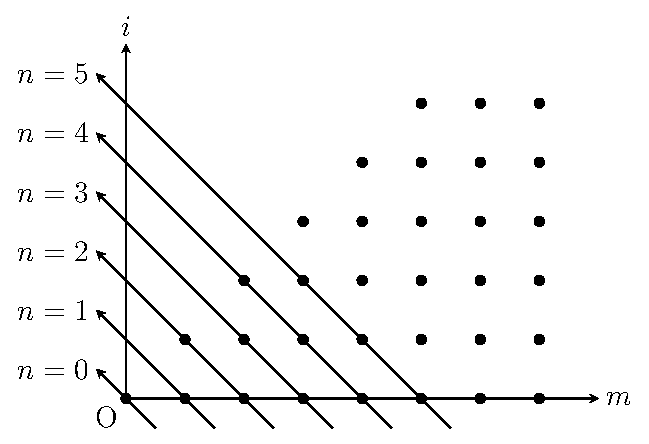
\includegraphics[width=60mm]{../TikZ/hermite/hermite.pdf}
    \caption{二重和の取りかえ方}
    \label{fig:hermite}
 \end{minipage}
  \end{tabular}
\end{figure}

\begin{equation*}
  g(t, x) = \sum_{n=0}^\infty \sum_{i=0}^{\lfloor \frac{n}{2} \rfloor} t^{n} \, (-1)^i
			\frac{1}{i! (n-2i)!} (2x)^{n-2i} 
\end{equation*}
これと母関数\eqref{eq:Hn-gene}の右辺を比較することで次を得る。
\begin{equation*}
  H_n(x) = \sum_{i=0}^{\lfloor \frac{n}{2} \rfloor} (-1)^i \frac{n!}{i! (n-2i)!} (2x)^{n-2i}
\end{equation*}\qed

\paragraph{母関数 $\Longrightarrow$ 漸化式}
母関数\eqref{eq:Hn-gene}の左、右辺を$t$で偏微分して
\begin{equation}\label{eq:Hn-gene->req-En}
  \frac{\6 g(t, x)}{\6 t} = \sum_{n=1}^\infty \frac{t^{n-1}}{(n-1)!} H_n(x)
	= \sum_{n=0}^\infty \frac{t^n}{n!} H_{n+1}(x)
\end{equation}
一方、母関数\eqref{eq:Hn-gene}の左、中辺を$t$について偏微分することで
\begin{equation*}
  \frac{\6 g(t, x)}{\6 t} = (-2t + 2x) g(t, x)
\end{equation*}
が成立することが分かる。これに母関数\eqref{eq:Hn-gene}の右辺および\eqref{eq:Hn-gene->req-En}を
代入すると、
\begin{gather*}
  \sum_{n=0}^\infty \frac{t^n}{n!} H_{n+1}(x)
	=  (-2t + 2x) \sum_{n=0}^\infty \frac{t^n}{n!} H_n(x) \notag\\
  \sum_{n=0}^\infty \frac{t^n}{n!} H_{n+1}(x)
	= -2 \sum_{n=0}^\infty \frac{t^{n+1}}{n!} H_n(x) 
		+ 2x \sum_{n=0}^\infty \frac{t^n}{n!} H_n(x) 
\end{gather*}
ここで$\frac{1}{(負の整数)!}= 0
\footnote{これは正でない整数$n$について$\Gamma(n) \ (= (n-1)! )$が発散することからの類推である。}
$と約束して$t$の指数をそろえると
\begin{gather*}
  \sum_{n=0}^\infty \frac{t^n}{n!} H_{n+1}(x)
	= -2 \sum_{n=0}^\infty \frac{t^n}{(n-1)!} H_{n-1}(x) 
		+ 2x \sum_{n=0}^\infty \frac{t^n}{n!} H_n(x) \notag\\
  \therefore \sum_{n=0}^\infty \frac{t^n}{n!}
	\[ H_{n+1}(x) - 2x H_n(x) + 2n H_{n-1}(x) \] = 0
\end{gather*}
$t^n \ (n \geq 0)$の係数を比較することで次を得る:
\begin{equation*}
  H_{n+1}(x) = 2x H_n(x) - 2n H_{n-1} (x)
\end{equation*}\qed

\paragraph{母関数 $\Longrightarrow$ 下降演算子}

母関数\eqref{eq:Hn-gene}の両辺を$x$で偏微分すると
\begin{equation*}
  \frac{\6 g(t, x)}{\6 x} = 2t \, g(t, x) = \sum_{n=0}^\infty \frac{t^n}{n!} H_n^\prime (x)
\end{equation*}
$g(t, x)$に母関数\eqref{eq:Hn-gene}の右辺を代入すると、
\begin{gather*}
  2t \sum_{n=0}^\infty \frac{t^n}{n!} H_n (x)
	= \sum_{n=0}^\infty \frac{t^n}{n!} H_n^\prime (x) \qquad \therefore
  2 \sum_{n=0}^\infty \frac{t^{n+1}}{n!} H_n (x)
	= \sum_{n=0}^\infty \frac{t^n}{n!} H_n^\prime (x) \notag
\end{gather*}
$\frac{1}{(負の整数)!}= 0$と約束して$t$の指数をそろえると
\begin{gather*}
  2 \sum_{n=0}^\infty \frac{t^{n}}{(n-1)!} H_{n-1} (x)
	= \sum_{n=0}^\infty \frac{t^n}{n!} H_n^\prime (x) \qquad \therefore
  \sum_{n=0}^\infty \frac{t^{n}}{n!} \[ H_n^\prime (x) - 2n H_{n-1} (x) \] = 0
\end{gather*}
$t^n \ (n \geq 0)$の係数を比較することで次を得る:
\begin{equation*}
  \dx{} H_n (x) = 2n H_{n-1} (x)
\end{equation*}\qed

\paragraph{漸化式, 下降演算子 $\Longrightarrow$ 上昇演算子}
漸化式\eqref{eq:Hn-req}と下降演算子\eqref{eq:Hn-kako}から
$2n H_{n-1}(x)$を消去することで直ちに
\begin{equation*}
  \( \dx{} -2x \) H_n(x) = - H_{n+1}(x)
\end{equation*} \qed

\paragraph{昇降演算子 $\Longrightarrow$ 微分方程式}

下降演算子の式\eqref{eq:Hn-kako}で$n \to n+1$とした式
\begin{equation}\label{eq:Hn-shoko->diff-En}
  \dx{} H_{n+1} (x) = 2(n+1) H_n(x)
\end{equation}
を用いるために、上昇演算子の式\eqref{eq:Hn-josho}の両辺に$\dx{}$を左から作用させると、
\begin{equation*}
  \dx{} \( \dx{} -2x \) H_n(x) = - \dx{} H_{n+1}(x)
\end{equation*}
演算子$f$について$\(\dx{}\) f = f \dx{} + \frac{df}{dx}  $であることなどに注意して左辺を展開し、
右辺に\eqref{eq:Hn-shoko->diff-En}を代入して整理すると
\begin{gather*}
  \( \dx{2} - 2x \dx{} -2 \) H_n(x) = - 2(n+1) H_n(x) \qquad \therefore
  \frac{d^2 H_n(x)}{dx^2} - 2x \frac{d H_n(x)}{dx} + 2n H_n(x) = 0 
\end{gather*}
また、この方程式は次のようにも変形できる。
\begin{equation*}
  \dx{} \( e^{-x^2} \dx{}H_n(x) \) + 2n  e^{-x^2} H_n(x) = 0
\end{equation*}\qed


\paragraph{母関数 $\Longrightarrow$ 直交性}

母関数\eqref{eq:Hn-gene}の右辺を用いて、
\begin{align}
  \int_{-\infty}^\infty e^{-x^2} g(s, x) g(t, x) \, dx
	&= \int_{-\infty}^\infty e^{-x^2} 
		\( \sum_{m=0}^\infty \frac{s^m}{m!} H_m(x) \) 
			\( \sum_{n=0}^\infty \frac{t^n}{n!} H_n(x) \) dx \notag\\
	&= \sum_{m=0}^\infty \sum_{n=0}^\infty \frac{s^m t^n}{m! n!}
		\int_{-\infty}^\infty e^{-x^2} H_m(x) H_n(x) \, dx
	\label{eq:Hn-gene->chokko-En1}
\end{align}
一方、母関数\eqref{eq:Hn-gene}の中辺を用いると
\begin{alignat}{2}
  \int_{-\infty}^\infty e^{-x^2} g(s, x) g(t, x) \, dx
	&= \int_{-\infty}^\infty e^{-x^2} e^{-s^2 + 2xs} e^{-t^2+2xt} dx \notag\\
	&= e^{-s^2-t^2} \int_{-\infty}^\infty e^{-x^2 + 2(s+t)x} dx \notag\\
	&= e^{-s^2-t^2} \int_{-\infty}^\infty e^{-\{ x-(s+t) \}^2} e^{(s+t)^2} dx \notag\\
	&= e^{2st} \int_{-\infty}^\infty e^{-\{ x-(s+t) \}^2} dx \notag\\
	&= e^{2st} \sqrt{\pi}  && (ガウス積分を用いた)\notag\\
	&= \sum_{n=0}^\infty \frac{2^n s^n t^n}{n!} \sqrt{\pi} && (\mathrm{Taylor}展開) \notag\\
	&= \sum_{m=0}^\infty \sum_{n=0}^\infty \frac{s^m t^n}{m! n!}
		\cdot 2^n n! \sqrt{\pi} \, \delta_{mn}
	\label{eq:Hn-gene->chokko-En2}
\end{alignat}
\eqref{eq:Hn-gene->chokko-En1}, \eqref{eq:Hn-gene->chokko-En2}を比較することで次を得る。
\begin{equation*}
  \int_{-\infty}^\infty e^{-x^2} H_m(x) H_n(x) \, dx = 2^n n! \sqrt{\pi} \, \delta_{mn}
\end{equation*}\qed

\end{document}